\documentclass[11pt]{article}
\usepackage{acl}
\usepackage{times}
\usepackage{latexsym}
\usepackage[T1]{fontenc}
\usepackage[utf8]{inputenc}
\usepackage{microtype}
\usepackage{inconsolata}
\usepackage{graphicx}
\usepackage{booktabs}
\usepackage{amsmath}
\usepackage{url}

\graphicspath{{figures/}}
\setlength\titlebox{6cm}

\title{What Should a Coding Agent Keep?\\Comparing Context Compaction Artifacts for Task Continuity}

\author{Joshua Liu \\
  University of California, Merced \\
  \texttt{jliu346@ucmerced.edu}}

\begin{document}
\maketitle

\begin{abstract}
Long-running coding agents eventually outgrow the model's working context, so systems must save earlier history in a shorter text summary (a \emph{memory artifact}). However, it is still unclear what artifact format best helps the model resume work correctly. We present a controlled continuation benchmark with 30 synthetic coding-session tasks across three families: constraint updating, exact-match retention, and workflow resumption. We compare five conditions: the full transcript, recent-turn truncation, an unstructured bullet summary, a structured state sheet, and a hybrid state sheet with exact preserved details. On a local \texttt{qwen3.5:4b} model served through Ollama, recent-only truncation falls to a task continuity score of 0.833, and the bullet summary reaches 0.920. In contrast, the structured state sheet matches the full transcript at 1.000 while using 26.6\% fewer prompt tokens. A same-family \texttt{qwen3.5:9b} robustness run shows the same ranking. The remaining errors are concentrated in file routing for the bullet summary, while the structured sheet alone saturates this benchmark, making extra exact-detail blocks unnecessary for standard context recovery on this task set. These results suggest that structured state sheets are a strong default memory artifact for coding agents, while coarser freeform summaries remain vulnerable to stale-file confusion.
\end{abstract}

{\raggedright
\noindent\textbf{Code and data availability:} \url{https://github.com/NumerousJLs/context-compaction-paper}\par
}

\section{Introduction}
Coding agents increasingly operate over long, tool-heavy sessions rather than short single-turn prompts. Prior work shows that long conversational state is difficult for large language models to preserve, both in dialogue-style settings and in multi-turn retrieval or agent tasks \citep{maharana-etal-2024-evaluating, jia-etal-2025-evaluating, katsis-etal-2025-mt}. The research community has responded with benchmarks, prompt compression methods, and full memory architectures \citep{chuang-etal-2024-learning, jeong-etal-2025-ecorag, kang-etal-2025-memory, hu-etal-2025-hiagent, sun-etal-2026-h}.

Even when prompt caching makes long contexts economically cheaper to reuse, keeping the full transcript eventually slows the workflow and makes it harder for the model to focus on the right earlier details. Practical systems therefore shrink older history before continuing the session. We use \emph{context compaction} as the umbrella term for that operation. In this paper, \emph{truncation} means deleting older turns, \emph{summarization} means rewriting older turns into freeform natural language, and a \emph{memory artifact} means the text block that survives compaction and is fed back to the model.

This design choice matters because resumed coding sessions depend on a mix of general state and precise syntax details. A useful memory artifact must preserve the current goal, the correct file to edit, the latest corrected constraint, and exact strings such as commands, environment variables, or failing test IDs. If the artifact is too abstract, the model loses its place in the codebase; if it is too detailed, the token savings become negligible.

We study this tradeoff with a narrow, controlled question: under a fixed compaction budget, what memory-artifact format best preserves task continuity in coding-style sessions? Rather than proposing a new learned memory system, we compare five interpretable conditions: the full transcript, recent-turn truncation, an unstructured bullet summary, a structured state sheet, and a hybrid state sheet plus exact details. Our focus is not whether compaction is useful in general, which is already well established, but which \emph{text representation} preserves the most actionable state per unit of context.

Our final results are clear and practically useful. First, naive truncation is too lossy, especially on hard cases where the recent turns contain a stale but plausible reminder. Second, coarse freeform summaries recover much of the lost state but still make file-routing mistakes. Third, structured state sheets remove those failures and match the full transcript with fewer prompt tokens. Finally, the hybrid exact-detail block does not improve over the structured sheet on our benchmark, suggesting that a well-structured state representation can already capture the needed continuation signal.

\section{Related Work}
\paragraph{Long-term memory and multi-turn continuity.}
Long-context and long-memory failures are already well documented. \citet{maharana-etal-2024-evaluating} introduce LoCoMo, a benchmark for very long-term conversational memory, while \citet{jia-etal-2025-evaluating} show that memory quality varies by information type over long spans. In retrieval-augmented dialogue, \citet{katsis-etal-2025-mt} show that preserving state across turns remains challenging.

\paragraph{Prompt and context compression.}
Context compaction itself is also an active area. \citet{chuang-etal-2024-learning} learn prompt compression in natural language formats, and \citet{jeong-etal-2025-ecorag} study evidentiality-guided compression for long-context RAG. These papers motivate budget-aware context reduction, but they do not directly answer the memory-artifact design question we ask here for coding-session continuation.

\paragraph{Structured memory and memory architectures.}
Several recent papers argue that structure matters for memory. \citet{hwang-etal-2024-enhancing} improve incremental summarization with structured representations, while \citet{kang-etal-2025-memory}, \citet{hu-etal-2025-hiagent}, and \citet{sun-etal-2026-h} propose richer multi-level memory architectures for long-horizon agents. Our work is deliberately smaller in scope: we compare frozen compact text artifacts rather than learned or hierarchical memory systems.

\section{Benchmark and Artifact Design}
\subsection{Task Design}
We build a synthetic continuation benchmark with 30 coding-session tasks. The goal is not to approximate all of software engineering, but to isolate common failure modes of long-running coding sessions in a form that can be scored quickly and reproducibly.

The three task families are benchmark-design choices rather than borrowed labels, but they are motivated by the same long-horizon memory and continuation pressures emphasized in prior conversational-memory and multi-turn evaluation work \citep{maharana-etal-2024-evaluating, jia-etal-2025-evaluating, katsis-etal-2025-mt}. We therefore choose families that stress changing rules, exact-string retention, and workflow continuation inside coding-style sessions.

These 30 tasks were drafted with \texttt{gpt-5.4} and manually refined by the author to keep the failure modes tightly controlled.

The benchmark has three task families, with 10 tasks per family:
\begin{itemize}
    \item \textbf{Constraint updating}: the session includes an earlier stale plan and a later correction that must override it.
    \item \textbf{Exact-match retention}: success depends on remembering an exact command, environment variable, regex, key format, or similar precise syntax detail.
    \item \textbf{Workflow resumption}: earlier setup work is already finished, so the correct continuation must avoid repeating completed work.
\end{itemize}

Six of the 30 tasks are harder variants. In these variants, the recent turns contain a stale but plausible reminder that points to an outdated file, rule, detail, or next step. This lets us test whether compacted memory can override misleading recency.

Each task contains a transcript prefix, followed by recent turns. We compact only the prefix. Every task also includes five candidate sets, one each for the active goal, target file, latest constraint, key exact detail, and next step. The model must return a candidate ID for each field.

\subsection{Artifact Conditions}
We compare five conditions:
\begin{itemize}
    \item \textbf{C0 Full transcript}: the full prefix plus recent turns.
    \item \textbf{C1 Recent only}: only the recent turns, with no compacted memory.
    \item \textbf{C2 Bullet summary}: an unstructured bullet summary of the earlier session.
    \item \textbf{C3 Structured state sheet}: explicit labeled fields for goal, status, file, constraint, open issue, and a generic next-step note.
    \item \textbf{C4 Hybrid state sheet}: the structured state sheet plus an exact-detail block and an exact next-action line.
\end{itemize}

The first two conditions act as control baselines: C0 is the upper bound, and C1 simulates naive truncation. C2 represents freeform summarization, while C3 and C4 test whether explicit structure improves memory quality, consistent with prior evidence that structured representations can preserve information better than unconstrained summaries \citep{hwang-etal-2024-enhancing}. For C2--C4, we keep a matched 85-word compaction budget. The memory artifacts are frozen before evaluation so that the main experiment isolates \emph{artifact format} rather than the model's own summarization skill.

To isolate format from generation capability, the C2--C4 artifacts were drafted with \texttt{gpt-5.4}, manually checked, and then frozen before evaluation to simulate an ideal compaction step. We chose 85 words as a practical shared budget that fit all three artifact types on local runs; we do not claim that 85 words is the best possible operating point.

\section{Experimental Setup}
\paragraph{Models and decoding.}
We run the main benchmark with the local \texttt{qwen3.5:4b} model served through Ollama, and we run a same-family \texttt{qwen3.5:9b} robustness check on the full benchmark. Decoding uses temperature 0, short JSON outputs only, and Ollama's non-thinking mode for deterministic completion behavior.

\paragraph{Evaluation target.}
For each task and condition, the model returns strict JSON with five fields:
\texttt{goal\_id}, \texttt{file\_id}, \texttt{constraint\_id}, \texttt{detail\_id}, and \texttt{next\_step\_id}. This closed-choice design avoids the instability of free-form judging and makes exact-match scoring possible.

\paragraph{Metrics.}
Our primary metric is \textbf{Task Continuity Score}, the average accuracy across the five fields. We also report per-field accuracy, average prompt token count from Ollama's \texttt{prompt\_eval\_count}, and average end-to-end latency per call. Error analysis uses a small taxonomy of wrong-file, lost-constraint, lost-exact-detail, wrong-next-step, and blended-old-and-new-state failures.

\section{Results}
\begin{table}[t]
\centering
\small
\resizebox{\linewidth}{!}{
\begin{tabular}{lcccc}
\toprule
Condition & Continuity & Avg. Tokens & Avg. Latency (s) & Reduction \\
\midrule
C0 Full transcript & 1.000 & 701.7 & 4.34 & 0.0\% \\
C1 Recent only & 0.833 & 423.0 & 3.57 & 39.7\% \\
C2 Bullet summary & 0.920 & 528.8 & 3.85 & 24.6\% \\
C3 Structured sheet & 1.000 & 515.1 & 3.82 & 26.6\% \\
C4 Hybrid sheet & 1.000 & 556.7 & 3.94 & 20.7\% \\
\bottomrule
\end{tabular}
}
\caption{Main results on \texttt{qwen3.5:4b}. ``Continuity'' is Task Continuity Score, the average accuracy across the five recovered fields. ``Avg. Latency'' is mean end-to-end seconds per call. ``Reduction'' is prompt-token reduction relative to C0. The structured sheet matches the full transcript while using fewer prompt tokens than the other compact artifacts.}
\label{tab:main}
\end{table}

Table~\ref{tab:main} and Figure~\ref{fig:main-results} show the main pattern. Recent-turn truncation is the weakest condition, dropping to a continuity score of 0.833. The coarse bullet summary recovers much of the lost state, but still trails at 0.920. Both the structured and hybrid artifacts match the full transcript at 1.000.

Context efficiency yields a similar advantage. Compared with the full transcript, the structured state sheet reduces average prompt tokens by 26.6\% while preserving perfect continuity. It also uses fewer prompt tokens than the bullet summary and the hybrid sheet, and it slightly reduces average end-to-end latency relative to the full transcript and the hybrid condition. Even if cached prefixes reduce repeated prefill cost, a shorter active context still lowers the amount of text the model must attend to when it chooses the next action. On this benchmark, the structured sheet is therefore the best cost/performance point rather than merely the highest-accuracy compact artifact.

Because our dataset is restricted to 30 highly curated tasks, these mean accuracy scores do not provide the statistical variance needed to cleanly separate closely performing conditions. A larger benchmark would allow confidence intervals or significance testing for tighter comparisons.

\begin{figure}[t]
\centering
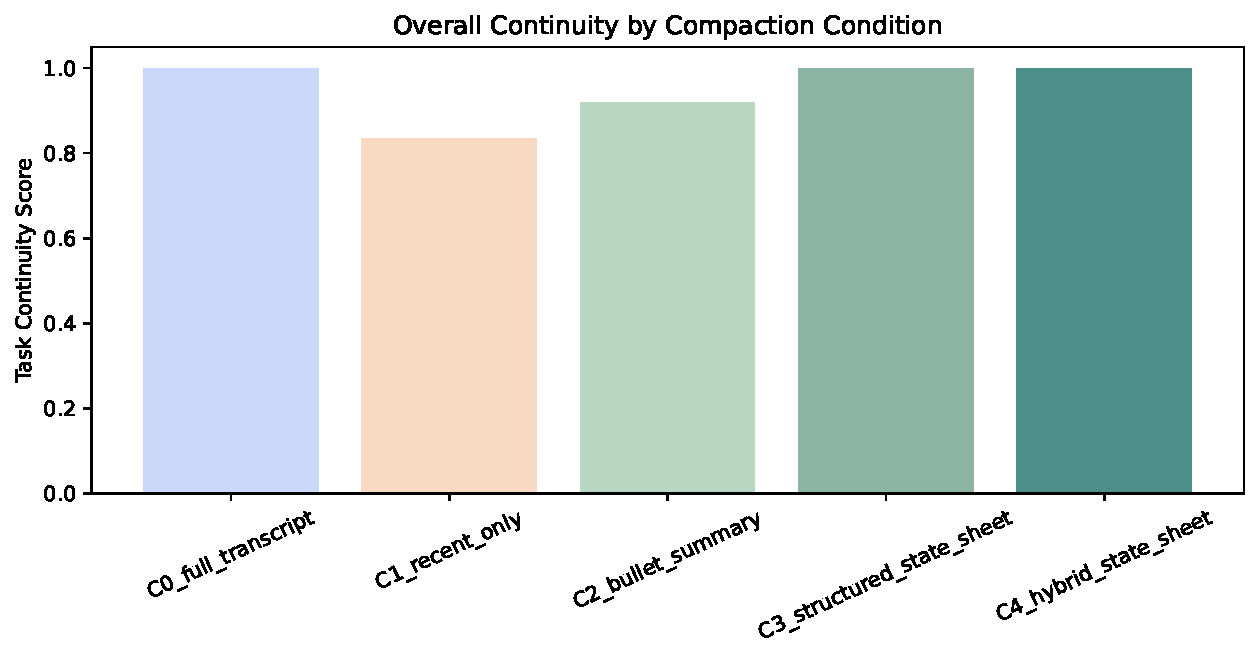
\includegraphics[width=\linewidth]{main_results.pdf}
\caption{Overall task continuity by condition on the \texttt{qwen3.5:4b} main run.}
\label{fig:main-results}
\end{figure}

\begin{figure}[t]
\centering
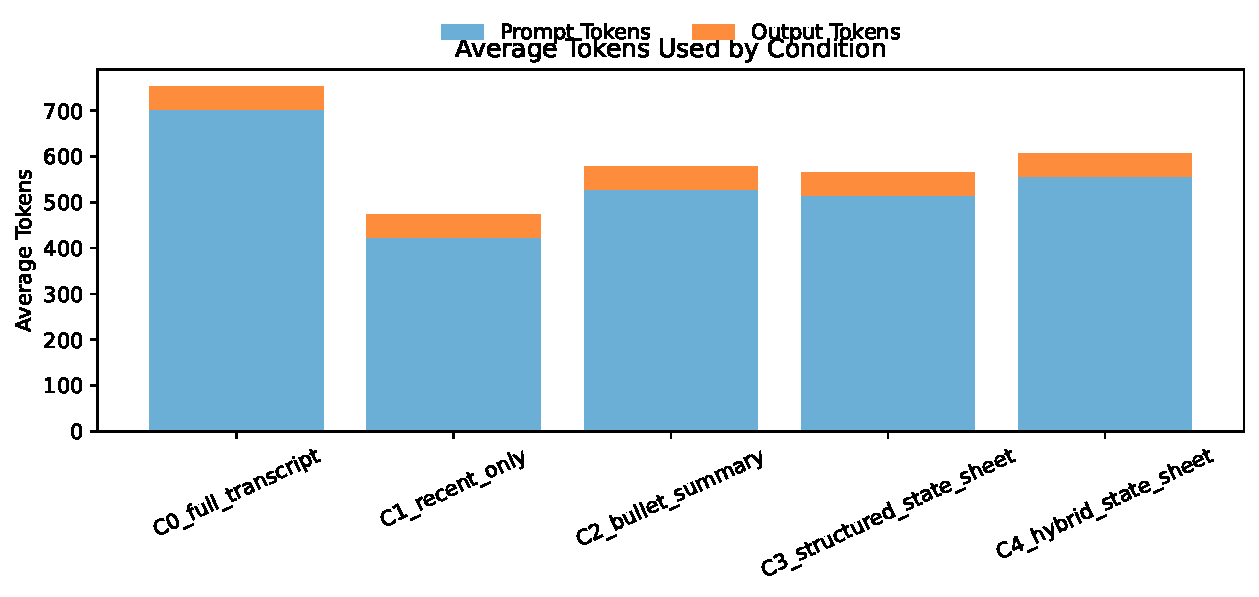
\includegraphics[width=\linewidth]{avg_tokens_by_condition.pdf}
\caption{Average prompt and output tokens by condition on the \texttt{qwen3.5:4b} main run. Output length is stable because the model returns short JSON predictions, so prompt design drives the token differences.}
\label{fig:avg-tokens}
\end{figure}

\subsection{Ablation Analysis: The Impact of Structure}
The per-field breakdown in Figure~\ref{fig:metric-breakdown} makes the tradeoff clearer. For \texttt{qwen3.5:4b}, the bullet summary preserves goals, constraints, details, and next steps very well, but file accuracy falls to 0.700. This is consistent with the artifact design: the bullet summary intentionally stores a coarser freeform description of the earlier session and omits the exact file path. In contrast, the structured sheet and hybrid sheet keep file accuracy at 1.000 because the target file is stored explicitly.

\begin{figure}[t]
\centering
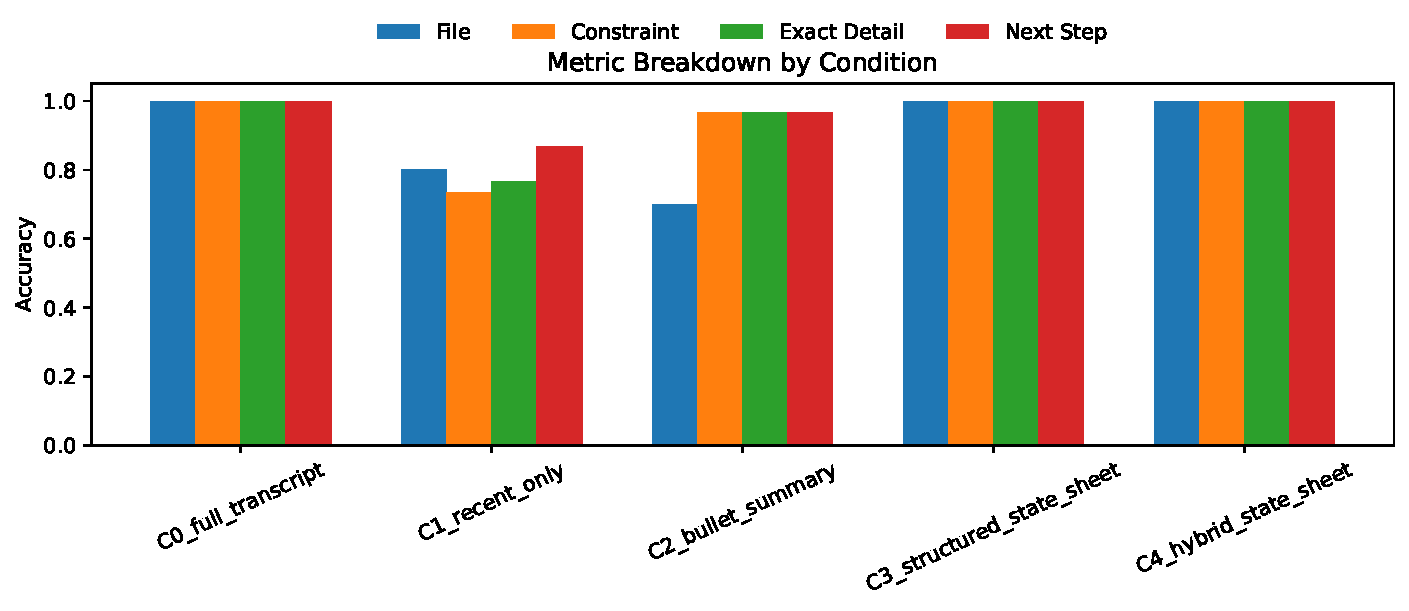
\includegraphics[width=\linewidth]{metric_breakdown.pdf}
\caption{Per-field accuracy by condition on the \texttt{qwen3.5:4b} main run. File retention is the main separation point between the coarse bullet summary and the structured artifacts.}
\label{fig:metric-breakdown}
\end{figure}

Comparing C2 to C3 shows the main structural ablation in this paper: once we replace a coarse freeform summary with an explicit schema, file routing errors disappear. By ablating the exact-detail block (comparing C4 to C3), we verify that additional raw details do not improve performance once the core schema is explicit. This is an informative negative result. It suggests that once the artifact stores the exact file, exact constraint, and open issue in a consistent schema, the model can already recover the remaining state without an extra explicit detail block.

\subsection{Hard vs. Easy Subsets}
The hard variants amplify the difference between truncation and compact memory. On the \texttt{qwen3.5:4b} run, recent-only truncation scores 0.917 on the easy subset but only 0.500 on the hard subset. The bullet summary also drops, from 0.950 to 0.800. When recent turns contain misleading information, freeform summaries fail to keep the model on track. In contrast, the structured artifacts remain at 1.000 on both subsets. This is strong evidence that the benchmark is not merely rewarding generic task recall: the memory artifact matters most when recent turns actively mislead the model.

\subsection{Model-Size Robustness}
\begin{table}[t]
\centering
\small
\begin{tabular}{lcccc}
\toprule
Model & C1 & C2 & C3 & C4 \\
\midrule
\texttt{4B} & 0.833 & 0.920 & 1.000 & 1.000 \\
\texttt{9B} & 0.920 & 0.960 & 1.000 & 1.000 \\
\bottomrule
\end{tabular}
\caption{Same-family robustness on the full 30-task benchmark. Larger model size improves the weaker compact artifacts, but the ranking stays the same.}
\label{tab:robustness}
\end{table}

Table~\ref{tab:robustness} shows the same-family robustness result. Moving from \texttt{qwen3.5:4b} to \texttt{qwen3.5:9b} improves the weaker conditions, especially recent-only truncation and the bullet summary, but does not change the ranking. The larger model is better at recovering state from partial context, yet the structured sheet remains the best compact artifact and the hybrid sheet still offers no measurable gain over it.

\section{Error Analysis}
\begin{figure}[t]
\centering
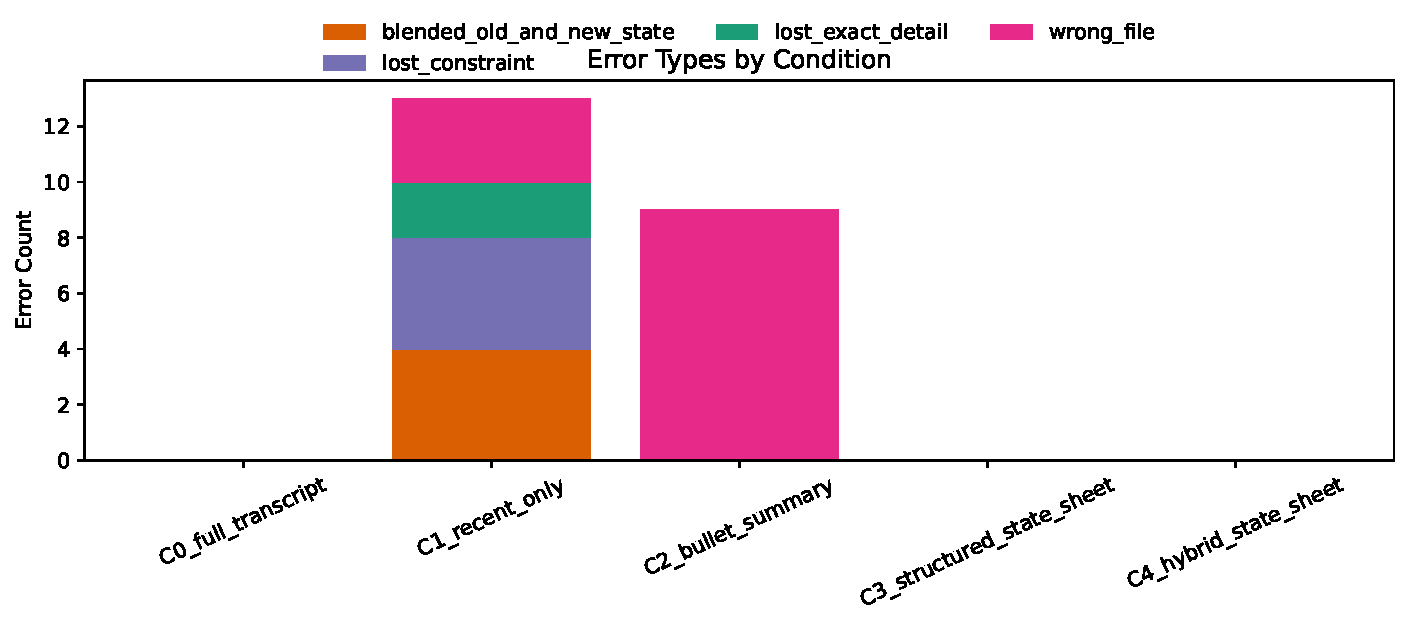
\includegraphics[width=\linewidth]{error_types.pdf}
\caption{Observed error types by condition on the \texttt{qwen3.5:4b} main run. The coarse bullet summary mainly fails by selecting the wrong file, while recent-only truncation mixes stale and current state.}
\label{fig:error-types}
\end{figure}

Figure~\ref{fig:error-types} summarizes the error types on the \texttt{qwen3.5:4b} run. Recent-only truncation fails in several ways: 4 blended-old-and-new-state cases, 4 lost-constraint cases, 3 wrong-file cases, and 2 lost-exact-detail cases. This is the expected failure mode when earlier state disappears and the model overweights the recent turns.

The bullet summary is substantially stronger overall, but its remaining errors are highly concentrated: all 9 bullet-summary failures are \texttt{wrong\_file} cases. For example, in the hard billing webhook task, the coarse summary preserves the goal, the corrected rule, the test detail, and the right next step, but still selects the stale schema file instead of \texttt{billing/webhook\_consumer.py}. In other words, the freeform summary keeps the overall story but loses the routing anchor.

The structured and hybrid artifacts make no errors on either full run. In this benchmark, explicit file and constraint slots are enough to remove the recurring failure pattern.

\section{Discussion}
The final result is slightly different from our original expectation. We initially hypothesized that the hybrid exact-detail block would outperform the structured sheet. Instead, the structured sheet already captures enough actionable state to match the full transcript on both models, and the extra exact-detail block provides no measurable gain on this benchmark while increasing token cost. This is still a useful design conclusion: if the benchmark is representative, the first compaction upgrade a coding agent should adopt is not a larger memory artifact, but a better schema.

The broader lesson is that freeform summaries and structured summaries fail differently. Coarse freeform memory is strong when the task only needs a generic story of what was happening, but it is weaker once the continuation depends on the correct file-level routing. Structured memory is more resilient precisely because it makes that routing information explicit.

\section{Limitations}
We restricted the benchmark to \textbf{N=30 tightly controlled tasks} to prioritize strict manual verification of complex multi-turn dependencies, plausible stale reminders, and compact artifacts before evaluation. Unlike math or short QA benchmarks that can be procedurally generated at scale, these continuation tasks required human checking to ensure the hard variants remained realistic rather than turning into generic retrieval prompts. The hard/easy splits and robustness checks support the main findings, but a sample size of 30 still means that small differences can come down to single-task variation. Other limitations include:
\begin{itemize}
    \item \textbf{Synthetic tasks:} The tasks isolate realistic failure modes, but they do not replace live coding-agent evaluation in an actual repository or tool loop.
    \item \textbf{Model diversity:} We evaluate only the \texttt{qwen3.5} family rather than a broad set of architectures and providers.
    \item \textbf{LLM-authored benchmark artifacts:} The compact artifacts were drafted with \texttt{gpt-5.4}, then reviewed and frozen before evaluation. This isolates representation quality, but future work must test whether deployed models can reliably generate C3-style schemas themselves.
    \item \textbf{Construction-model bias:} The tasks and compact artifacts were both created during a \texttt{gpt-5.4}-assisted benchmark-writing process. Although the evaluation models are from the separate \texttt{qwen3.5} family, future work should test whether the same findings hold on fully human-written or independently sourced continuation data.
    \item \textbf{Closed-choice evaluation:} By asking the model to return candidate IDs rather than generate file paths or next actions freely, we simplify the continuation task and reduce open-ended hallucination. This likely contributes to the ceiling effect for C3 and C4.
    \item \textbf{Positional bias constraints:} In C3 and C4, the compacted memory appears before the recent turns. Prior work on primacy and recency effects suggests that artifact placement within the prompt may matter, so future work should test whether these results hold when the memory block moves within the context window.
    \item \textbf{Single compaction budget:} We use one 85-word budget rather than a scaling curve over multiple budgets, so we do not claim that the current separation would stay identical at 40 or 200 words.
    \item \textbf{Top-end ceiling effects:} Both models saturate on C3 and C4, with both conditions reaching 1.000 on the full benchmark. A stricter benchmark with more tasks and harder top-end distinctions is needed to test whether structured memory and exact-detail memory ever separate under more rigorous conditions.
\end{itemize}

\section{Conclusion}
We presented a controlled study of context compaction artifacts for coding-session continuation. The results are simple but useful: truncation is too lossy, coarse bullet summaries recover most of the state but still lose file routing, and structured state sheets match the full transcript while using fewer prompt tokens. In our benchmark, the structured sheet already saturates the task set, so the extra exact-detail block yields no measurable gain here. For local coding agents that need a practical compaction policy without new model training, explicit state structure appears to matter more than adding more raw detail on standard context-recovery tasks.

\bibliography{custom}

\appendix
\section{Prompt Templates and JSON Schema}
\label{sec:appendix_prompts}
To ensure reproducibility, we provide the exact prompt template and JSON schema used to query the \texttt{qwen3.5} models via Ollama.

\textbf{System Prompt:} No separate system prompt was used. All instructions were placed in a single user prompt with deterministic decoding (\texttt{temperature=0}, \texttt{think=false}).

\textbf{User Prompt Template:}
{\footnotesize
\begin{verbatim}
Recover the current coding-session state from the context below.
Use only the provided session context and recent turns.
Choose exactly one option ID for each field.
Return JSON only with these keys: goal_id, file_id, constraint_id,
detail_id, next_step_id.

[CONTEXT_BLOCK]

[CANDIDATE_TEXT]

Return strict JSON only.
\end{verbatim}
}

\textbf{Context Block Template:}
{\footnotesize
\begin{verbatim}
C0_full_transcript:
EARLIER SESSION:
[PREFIX_TURNS]

RECENT TURNS:
[RECENT_TURNS]

C1_recent_only:
RECENT TURNS ONLY:
[RECENT_TURNS]

C2/C3/C4:
COMPACTED MEMORY:
[ARTIFACT_TEXT]

RECENT TURNS:
[RECENT_TURNS]
\end{verbatim}
}

\textbf{Candidate-Set Format:}
{\footnotesize
\begin{verbatim}
GOAL OPTIONS:
  A: ...
  B: ...
  C: ...

FILE OPTIONS:
  A: ...
  B: ...
  C: ...

CONSTRAINT OPTIONS:
  A: ...
  B: ...
  C: ...

DETAIL OPTIONS:
  A: ...
  B: ...
  C: ...

NEXT_STEP OPTIONS:
  A: ...
  B: ...
  C: ...
\end{verbatim}
}

\textbf{JSON Schema:}
{\footnotesize
\begin{verbatim}
{
  "goal_id": "A|B|C",
  "file_id": "A|B|C",
  "constraint_id": "A|B|C",
  "detail_id": "A|B|C",
  "next_step_id": "A|B|C"
}
\end{verbatim}
}

\section{Example Run}
\label{sec:appendix_example}
Table~\ref{tab:example-run} shows one abbreviated example from the hard workflow-resumption family. In this task, the recent turns contain a stale reminder pointing to the wrong file and the wrong next action. The recent-only condition follows that stale reminder, while the structured state sheet recovers the correct file and next step.

\begin{table}[t]
\centering
\small
\resizebox{\linewidth}{!}{
\begin{tabular}{p{0.26\linewidth}p{0.68\linewidth}}
\toprule
Component & Content \\
\midrule
Recent stale reminder & ``work in \texttt{billing/webhook\_schema.py}'' and revisit the schema migration \\
Gold next action & edit \texttt{billing/webhook\_consumer.py} and handle the 409 retry path \\
C1 prediction & \{\texttt{file\_id: B}, \texttt{constraint\_id: A}, \texttt{detail\_id: B}, \texttt{next\_step\_id: A}\} \\
C3 prediction & \{\texttt{file\_id: A}, \texttt{constraint\_id: C}, \texttt{detail\_id: A}, \texttt{next\_step\_id: C}\} \\
\bottomrule
\end{tabular}
}
\caption{Abbreviated example from task \texttt{ns01\_hard}. The structured state sheet overrides the misleading recent reminder, while recent-only truncation follows it.}
\label{tab:example-run}
\end{table}

\end{document}
